\begin{figure}
 \centering
 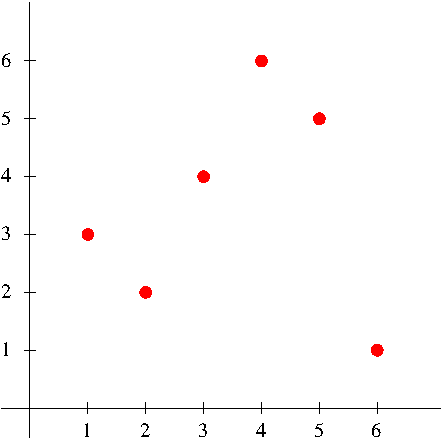
\includegraphics{Cmonextr_1.pdf}
 % Cmonextr_1.pdf: 212x210 pixel, 72dpi, 7.48x7.41 cm, bb=0 0 212 210
 \caption{Exemple}
 \label{fig:Cmonextr_1}
\end{figure}


\begin{enumerate}
 \item La figure \ref{fig:Cmonextr_1} aide à extraire les fonctions croissantes ou décroissantes.
\begin{enumerate}
 \item On trouve 12 parties $A$ contenant au moins deux éléments et telles que $f_A$ soit croissante. 
\begin{multline*}
 \{1,3\}, \{1,4\}, \{1,5\}, \{1,3,4\}, \{1,3,5\}, \{2,3,4\}, \{2,3\}\{2,4\}, \{3,4\},\\
 \{2,3,5\}, \{2,5\}, \{3,5\}
\end{multline*}
\item On trouve 9 parties $A$ contenant au moins deux éléments et telles que $f_A$ soit décroissante.
\begin{displaymath}
 \{1,2,6\},\{1,2\},\{1,6\},\{2,6\},\{3,6\},\{4,5,6\},\{4,6\},\{5,6\},\{4,5\}
\end{displaymath}
En cherchant ces parties, on réalise bien que certaines sont \emph{maximales}. Les questions suivantes précisent ce point.
\end{enumerate}
\item \begin{enumerate}
 \item La convention de l'énoncé relative aux restrictions à des singletons rend les questions 2.a et 3.a  évidentes. Pour chaque $p$, le singleton $\{p\}$ convient. Ces questions servent seulement à justifier que les parties de $\N$ dont on veut prendre les plus grands éléments sont non vides. Comme ces parties sont majorées par $m$, on est assuré de l'existence de ces plus grands éléments. Il s'agit de trouver la taille maximale des séquences croissantes ou décroissantes qui se terminent en $p$. \\
On présente directement le tableau des résultats en 3.c.
\item Voir 3.c
\end{enumerate}
\item \begin{enumerate}
 \item Voir 3.c 
\item Voir 3.c
\item Tableau des résultats comprenant les questions 2.b et 2.c.
\begin{center}
\renewcommand{\arraystretch}{1.3}
% use packages: array
\begin{tabular}{|l|c|c|c|c|c|c|}  \hline 
$p$ & 1 & 2 & 3 & 4 & 5 & 6 \\ \hline 
$i_p$ & 1 & 1 & 2 & 3 & 3 & 1 \\  \hline 
$j_p$ & 1 & 2 & 1 & 1 & 2 & 3 \\ \hline
$(i_p,j_p)$ & $(1,1)$ & $(1,2)$ & $(2,1)$ & $(3,1)$ & $(3,2)$ & $(1,3)$ \\ \hline
\end{tabular}
\end{center}
\hspace{.3cm}
\end{enumerate}

\item \begin{enumerate}
 \item Soit $p<q$ et $A$ une partie de cardinal $i_p$ vérifiant les conditions de 2.a pour $p$. Lorsque $f(p)<f(q)$, on peut adjoindre $q$ à $A$. Alors la restriction de $f$ à $A\cup \{q\}$ est toujours croissante et $A\cup \{q\}$ vérifie les conditions de 2.a relatives à $q$. On en déduit :
\begin{displaymath}
 i_q \geq i_p + 1
\end{displaymath}
\item Le raisonnement est analogue à celui de la question précédente.
\end{enumerate}

\item Notons $\varphi$ l'application définie dans $E$ par $\varphi(p)=(i_p,j_p)$.\\
Supposons $\varphi(p)=\varphi(q)$ avec $p<q$.\\
Comme $i_p=i_q$, l'inégalité $i_p < i_q$ est fausse. Donc, d'après 4.a., l'inégalité $f(p)<f(q)$ l'est aussi. On en déduit
\begin{displaymath}
 f(q) \leq f(p)
\end{displaymath}
De même, comme $j_p<j_q$ est fausse, $f(q)<f(p)$ l'est aussi donc $f(p)\leq f(q)$.\\
On en déduit donc $f(p)=f(q)$ puis $p=q$ à cause de l'injectivité de $f$.
\item \emph{Théorème de Erdös-Szekeres}. Conservons la notation $\varphi$ de la question précédente.\\
Comme $\varphi$ est injective, elle prend $m$ valeurs distinctes. Il est donc impossible que ces valeurs (qui sont des couples) soient \emph{toutes} dans le produit cartésien
\begin{displaymath}
 \{1,2,\cdots,a\}\times\{1,2,\cdots,b\}
\end{displaymath}
qui en contient seulement $ab$ avec $ab<ab+1=m$.\\
On en déduit qu'il existe un $p$ tel que $i_p>a$ ou tel que $j_q>b$. Dans le premier cas, il existe une partie $A$ contenant strictement plus de $a$ éléments telle que $f_A$ soit croissante. Dans le second cas, il existe une partie $B$ contenant strictement plus de $b$ éléments telle que $f_B$ soit décroissante.
\item \begin{enumerate}
 \item Commençons par mettre en évidence une partie $D$ telle que $f_D$ soit décroissante. Fixons un $m$ entre $0$ et $b-1$ et considérons
\begin{displaymath}
 D = \{ma,ma+1, \cdots,ma +(a-1)\}
\end{displaymath}
Elle contient $a$ éléments qui ont tous le même quotient $m$ dans la division par $a$ et des restes croissant de $0$ à $a-1$. La restriction à $D$ ne dépend que du reste et elle est décroissante.\\
Nous allons maintenant démontrer
\begin{displaymath}
 x<x' \text{ et } f(x) > f(x') \Rightarrow q(x)=q(x')
\end{displaymath}
En effet, d'une part
\begin{displaymath}
 x<x' \Rightarrow q(x)\leq q(x') \Rightarrow q(x')-q(x) \geq 0
\end{displaymath}
D'autre part,
\begin{multline*}
 f(x)>f(x') \Rightarrow r(x')-r(x) > (q(x')-q(x))a
\Rightarrow (q(x')-q(x))a < a \\
\Rightarrow q(x')-q(x) < 1
\end{multline*}
Dans $\Z$, les deux inégalités ne peuvent se produire que si $q(x)=q(x')$.\\
On en déduit que lorsque $f_A$ est décroissante, la partie $A$ est incluse dans une partie de la forme $D$. Elle contient donc au plus $a$ éléments.
\item Considérons maintenant une partie 
\begin{displaymath}
 C = \{k, a+k, 2a+k,\cdots ,(b-1)a+k\}
\end{displaymath}
pour un $k$ fixé entre $0$ et $a-1$. Elle contient $b$ éléments tous de même reste mais de quotients croissant de $0$ à $b-1$. La restriction de $f$ à $C$ ne dépend que du quotient, elle est donc strictement croissante.\\ Montrons maintenant
\begin{displaymath}
 x<x' \text{ et } f(x) < f(x') \Rightarrow q(x) < q(x')
\end{displaymath}
En exprimant $r(x)$ en fonction de $x$ et $q(x)$ on obtient
\begin{displaymath}
 f(x) = 2q(x)a + a - x
\end{displaymath}
On en déduit
\begin{displaymath}
 f(x')-f(x)= 2(q(x')-q(x)) -(x'-x)
\end{displaymath}
En particulier
\begin{displaymath}
 f(x')-f(x)>0 \Rightarrow 2(q(x')-q(x)) > x'-x
\end{displaymath}
Finalement:
\begin{displaymath}
 \left. 
\begin{aligned}
 x<&x'\\ f(x)<&f(x')
\end{aligned}
\right\rbrace 
\Rightarrow 2(q(x')-q(x)) > x'-x > 0 \Rightarrow q(x)<q(x')
\end{displaymath}
Si $A$ est une partie telle que $f_A$ soit croissante, on ne peut pas déduire que $A$ est de la forme de $C$. On sait que les quotients doivent croître mais on n'a pas prouvé que les restes sont les mêmes. Une telle partie doit donc être de la forme
\begin{displaymath}
 \{k_0, a+k_1, 2a+k_2,\cdots ,(b-1)a+k_{b-1}\}
\end{displaymath}
où les $k_i$ sont entre $0$ et $a-1$. Elle contient au plus $b$ éléments.
\item Les questions précédentes montrent qu'il existe un exemple de fonction $f$ définie dans un ensemble contenant $ab$ éléments avec lequel, pour toute partie $A$ : 
\begin{align*}
 f_A \text{ croissante } &\Rightarrow \sharp A \leq b \\
 f_A \text{ décroissante } &\Rightarrow \sharp A \leq a \\
\end{align*}
On ne peut donc pas étendre le théorème au cas où $m=ab$.
\end{enumerate}

\end{enumerate}
